% Sample LaTeX file for creating a paper in the Morgan Kaufmannn two
% column, 8 1/2 by 11 inch proceedings format.
% Thoughts on methodology
% 1. Evaluate action in local context (sequence).
% examples: shot is worth more in powerplay, second shot is worth more
% 2. Evaluate action with transition to penalty. Evaluates path from local context to penalty.
% 3. Evaluate action with arbitrary transition.
% to evaluate predictive power: instead of log-likelihood, could compute entropy.
% to replicate Shuckers: try using the average conditional probability difference over all states where an action is taken. don't see context = marginalize over context.
% convergence condition: update converges if the difference between player value increases goes to 0 as k goes to infinity. This expresses a certain symmetry in the game.
% questions for tim/Sloan 
%1. predict performance from one season to the next. E.g., does sum of impact predict next season 
%1a. What about evaluating action with respect to line? What about with respect to both players (e.g. in a hit).
%2. run regression on context for each action.
%3. evaluate what contributes to a penalty.
%4. evaluate special players. Compare model for each player vs. adding a player weight.

\documentclass[]{article}
\usepackage{proceed2e}

% Set the typeface to Times Roman
\usepackage{times}
\usepackage{url}
\usepackage[square]{natbib}
\usepackage{varwidth}
%Example for automatically rescaling equations. 
% This is very tricky.
%\begin{equation}
%\label{eq:pimax}
%\resizebox{.55\textwidth}{!}{$
%\begin{split}
%P(\jtable_{2}|\set{E},\ttable) \propto &
%P(\keys = [jack,101],\it{Gr} = A, \it{Sat} = 1|\it{Int} = \class, \it{Rank} = 1, \it{Rat} = 3, \it{Diff}=1)\\
%\times & P(\keys = [jack,102],\it{Gr} = B, \it{Sat} = 2|\it{Int} = \class, \it{Rank} = 1, \it{Rat} = 2, \it{Diff}=2).
%\end{split}$
%}
%\end{equation}

%\usepackage{times}
%\usepackage[normaltitle,normalbib,normalmargins,normalindent]{savetrees}
\usepackage{amsmath}
\usepackage{amsfonts}
\usepackage{amssymb}
\usepackage{graphicx}
\usepackage{url}
%\usepackage{subfigure}
\usepackage{epstopdf}
\setcounter{MaxMatrixCols}{30}
%\usepackage{algorithm}
%\usepackage{algorithmic}
\usepackage{subfigure}
%\usepackage{subcaption}
\usepackage{fancyhdr}
\graphicspath{{../}{figures/}}
\usepackage{todonotes}

\DeclareMathOperator*{\argmax}{argmax}
\DeclareMathOperator*{\argmin}{argmin}
%\DeclareMathOperator{\pattern}{\pi}
\DeclareMathOperator{\Poly}{\mathbf{\mathrm{P}}}
\DeclareMathOperator{\RP}{\mathbf{\mathrm{RP}}}
%\DeclareMathOperator{\FP}{\mathbf{\mathrm{FP}}}
\DeclareMathOperator{\NP}{\mathbf{\mathrm{NP}}}
%\DeclareMathOperator{\E}{\mathbb{E}}
\renewcommand{\d}{\mathbf{d}}

\newcommand{\ZZ}{\mathbf{Z}}

\newcommand{\indep}{\ensuremath{\perp{}\!\!\!\!\!\!\!\perp{}}}
\newcommand{\dep}{\ensuremath{{\perp{}\!\!\!\!\!\!\!\not  \perp{}}}}
%\renewcommand{\L}{\mathcal{L}}
% variables denoting sets of nodes
\newcommand{\V}{V} 
\newcommand{\partC}{\mathcal{C}}
\newcommand{\pattern}{\pi}
% variables denoting nodes
\newcommand{\B}{B}
\renewcommand{\P}{P}
\newcommand{\R}{R}
\newcommand{\X}{X}
\newcommand{\Y}{Y}
\newcommand{\Z}{Z}
\newcommand{\F}{F}
\newcommand{\U}{U}
\newcommand{\W}{W}
\renewcommand{\S}{S}
\newcommand{\C}{C}
\newtheorem{mydef}{Proposition}
%variables for values
%\newcommand{\u}{u}
\renewcommand{\a}{a}
\renewcommand{\b}{b}
\newcommand{\z}{z}
\renewcommand{\v}{v}
\newcommand{\x}{x}
\newcommand{\y}{y}
\newcommand{\p}{p}
\newcommand{\s}{s}
\newcommand{\w}{w} % weights


%statistics
\newcommand{\divergence}{\it{D}}
\newcommand{\score}{\it{score}}
\newcommand{\confidence}{\it{conf}}
\newcommand{\support}{\it{support}}
\newcommand{\loglikelihood}{\it{LOG}}
\newcommand{\lof}{\it{LOF}}
\newcommand{\llmetric}{-L}
\newcommand{\lr}{\it{LR}}
\newcommand{\kl}{\it{KL}}
\newcommand{\el}{\it{EL}}
\newcommand{\mi}{\it{MI}}
\renewcommand{\mid}{\it{ELD}}
\newcommand{\jid}{\it{JID}}
\newcommand{\roc}{\it{ROC}}
\newcommand{\outrank}{\it{OutRank}}
\newcommand{\knn}{\it{KNNOutlier}}
\newcommand{\auc}{\it{AUC}}
\newcommand{\eld}{\it{ELD}}
\newcommand{\fd}{\it{FD}}
\newcommand{\parameter}{\theta}
\newcommand{\parameters}{\bs{\parameter}}
\newcommand{\bic}{\mathit{BIC}}
%random variables and graphical models
% number of values in the domain of a random variable
% variables for BNs
\newcommand{\domvals}{k}
\newcommand{\nodevalue}{\v}
\newcommand{\parvalue}{\mathbf{\pi}} % a single assignment of values to a set of 
%parents
\newcommand{\parvals}{l} % number of values of parent state.
\renewcommand{\r}{r} % CP-table row
\newcommand{\nbhd}{{\mathsf {nbdh}}}
\newcommand{\child}{\mathit{child}}
\newcommand{\parent}{\mathit{pa}}
\newcommand{\parents}{\mathbf{pa}}
\newcommand{\Parents}{\mathbf{PA}}
\newcommand{\family}{F} % families, family formulas
\newcommand{\vpi}{\mathbf{pa}} % for vectors of variable assignments
\renewcommand{\l}{\ell} % class label
\newcommand{\states}{r} % number of states of a variable
%\newcommand{\value}{value}
\newcommand{\mb}{\set{mb}} % markov blanket of a variable, vector-valued
\newcommand{\ssize}{N} % number of rows in join table; size of sample
\newcommand{\mbstates}{m} % number of states in Markov blanket
\newcommand{\frequency}{fr}
\newcommand{\pseudo}{\ast}
\newcommand{\counts}{+}
\newcommand{\weighted}{\ast}
\newcommand{\halpern}{H}
\newcommand{\Thetaa}{\theta}
\newcommand{\instance}{I}

%logic notation
%\newcommand{\predicate}{\phi}
\newcommand{\functor}{f}
\newcommand{\outdomain}{V}
\newcommand{\indomain}{\Omega}
\newcommand{\variable}{X} % first-order variable
\newcommand{\population}{\mathcal{P}}
\newcommand{\entity}{x}
\newcommand{\formula}{\phi}
\newcommand{\formulas}{\mathcal{\phi}}
\newcommand{\literal}{l}
\newcommand{\conjunction}{\set{C}} % conjunction of literals
\newcommand{\fterm}{\f} % open function term
\newcommand{\fterms}{F} % set of function terms, also nodes in JBN
\newcommand{\term}{\sigma}
\newcommand{\Terms}{\bs{\sigma}}
\newcommand{\constant}{a}
\newcommand{\constants}{\bs{\constant}}
\newcommand{\gterm}{g} % ground term
\newcommand{\gterms}{\bs{\gterm}} %list of ground terms
\newcommand{\vterm}{x} % variable term
\newcommand{\vterms}{\bs{\vterm}} % list of variable terms
\newcommand{\assign}{A} % assignment of values to Bayes net
\newcommand{\resultset}{\mathbb{R}}
\newcommand{\grounds}{\#}
\newcommand{\grounding}{\gamma}
\newcommand{\groundall}{\Gamma}
\newcommand{\vars}{\mathit{Var}} % variables in a conjunction
\newcommand{\igraph}{I} % instance-level dependency graph.
\newcommand{\assignment}{\set{a}}
\newcommand{\atom}{\ell}
\newcommand{\gnode}{\alpha}
\newcommand{\gfamily}{\ground{f}}
\newcommand{\numformulas}{m}
\newcommand{\structure}{\mathcal{S}}
% logic programs
\newcommand{\program}{\mathcal{B}}
\newcommand{\clause}{\mathcal{c}}
\newcommand{\head}{\mathit{head}}
\newcommand{\body}{\mathit{body}}
\newcommand{\crule}{\mathit{cr}} % combining rule
\newcommand{\level}{\mathit{level}} % rank of function symbols in LP

%datbase schema
\newcommand{\rcolumns}{R}
\newcommand{\ecolumns}{E}
\newcommand{\dtable}{T} % can't use \table. Generic database table
\newcommand{\datatable}{D} % generic data table, not necessarily part of database.
\newcommand{\jtable}{J} % join table
\newcommand{\Ejoin}{$J^{+}$}
\newcommand{\jtables}{m}
\newcommand{\rtable}{R} % relationship table
\newcommand{\etable}{E} % entity table.
\newcommand{\ttable}{X} % target table
\newcommand{\nextended}{n}
\newcommand{\row}{r}
\newcommand{\rows}{\mathit{rows}}
\newcommand{\col}{j}
\newcommand{\cols}{\mathit{cols}}
\newcommand{\unary}{\f} % to denote a unary or attribute function
\newcommand{\numatts}{u} % to denote the number of unary or attribute functions.
\newcommand{\g}{g} % alternative for function
\newcommand{\relational}{\mathbf{r}} % denotes a generic relational functors, can be both relationship or descriptive attribute of relationship
\newcommand{\Relation}{R} % denotes a generic boolean relation
% a special type of literal conjunction that assigns a value %to each variable
\providecommand{\keywords}{\textbf{keywords: }}
\newcommand{\loss}{\ell}
\newcommand{\class}{c} % the class attribute
\newcommand{\classlabel}{y} % the class label
\newcommand{\classifier}{\mathcal{M}}
\newcommand{\target}{t} % target object
\newcommand{\Target}{T}
\newcommand*\rfrac[2]{{}^{#1}\!/_{#2}}
\newcommand{\object}{o}
\newcommand{\Class}{C}
\newcommand{\scorediff}{\Delta}
\newcommand{\model}{B}
\newcommand{\modelprob}{\theta}
\newcommand{\profile}{P}
% the probabilities defined by a model, like conditional probabilities in a BN
\newcommand{\Targetcount}{\Gamma}
\newcommand{\neighbor}{n}
\newcommand{\feature}{V} % feature or desc attribute of object or link
\newcommand{\features}{\bs{v}} % features 
\newcommand{\Features}{\bs{V}}
\newcommand{\attribute}{a} % nonclass attribute of target object
\newcommand{\attributes}{\bs{a}}
\newcommand{\rels}{\bs{R}} % chain of relationships.
\newcommand{\maxpath}{\rho}
\newcommand{\eatts}{\it{1Nodes}}
\newcommand{\ratts}{\it{2Nodes}}
\newcommand{\atts}{\it{ANodes}}
\newcommand{\marginalize}{\it{margin}}
%special functions
\newcommand{\AVG}{\it{AVG}}
\newcommand{\instances}{n} % counts number of occurrences in DB
\newcommand{\prob}{p} % frequency of formula true in in DB

%variables denoting graphs or models
\newcommand{\mln}{M}
\newcommand{\G}{G}
\newcommand{\node}{V}
\newcommand{\nodes}{V}
\newcommand{\edges}{E}
\newcommand{\clique}{C}
\newcommand{\cliques}{\mathcal{\clique}}
\newcommand{\cliquevalue}{c}
\newcommand{\graph}{G}
\newcommand{\M}{M}
\newcommand{\J}{J}
\renewcommand{\H}{H}
\newcommand{\K}{K} % component
\renewcommand{\O}{O} % oracle
\renewcommand{\path}{\rho} % path, also foreignkey path
% Markov nets
\newcommand{\potential}{\Psi}
% database schema
\newcommand{\type}{\tau} % to denote a generic type
\newcommand{\E}{E} % for entity tables
\newcommand{\e}{e} % for specific entities
\newcommand{\f}{f}
\newcommand{\new}{\it{new}}
\renewcommand{\c}{c}
\renewcommand{\R}{R} % for relationship tables
\newcommand{\A}{A} % for attributes
\newcommand{\T}{T} % for tables generically
\newcommand{\New}{N}
\newcommand{\D}{\mathcal{D}} % for database instance
\newcommand{\databases}{\set{D}} % the number of databases
\newcommand{\vocab}{\mathcal{\L}} % for logical vocabulary associated with database
\newcommand{\name}{\mathit{name}} % generic attribute
\newcommand{\dom}{\mathit{dom}} % domain of attributes
\newcommand{\etables}{\alpha} % entity tables
\newcommand{\rtables}{\beta} % relationship table number
% specific constructs for examples


\newcommand{\team}{\it{T}}
\newcommand{\player}{\it{P}}
\newcommand{\match}{\it{M}}


\newcommand{\director}{\it{Director}}
\newcommand{\movie}{\it{Movie}}
\newcommand{\user}{\it{User}}
\newcommand{\corr}{\it{\rho}}
\newcommand{\student}{\mathit{Student}}
\newcommand{\I}{\mathit{I}}
\newcommand{\course}{\mathit{Course}}
\newcommand{\prof}{\mathit{Professor}}
\newcommand{\person}{\mathit{Person}}
\newcommand{\TA}{\mathit{TA}}
\newcommand{\actor}{\mathit{Actor}}
\newcommand{\age}{\mathit{age}}
\newcommand{\intelligence}{\mathit{intelligence}}
\newcommand{\diff}{\mathit{difficulty}}
\newcommand{\reg}{\mathit{Registered}}
\newcommand{\win}{\it{win}}
\newcommand{\ra}{\mathit{RA}}
\newcommand{\bt}{\mathit{blood type}}
\newcommand{\grade}{\mathit{grade}}
\newcommand{\gpa}{\mathit{gpa}}
\newcommand{\jack}{\mathit{Jack}}
\newcommand{\jill}{\mathit{Jill}}
\newcommand{\smith}{\mathit{Smith}}
\newcommand{\cmpt}{\mathit{CMPT120}}
\newcommand{\hi}{\mathit{Hi}}
% various constants
\newcommand{\true}{\mathit{T}}
\newcommand{\false}{\mathit{F}}
\newcommand{\normalconstant}{Z} % the normalization constant

% orderings
\newcommand{\pred}{\mathit{pred}}
%procedure names and such
\newcommand{\join}{\textsc{Join-Frequencies}}
\newcommand{\linus}{\textsc{Linus }}
\newcommand{\foil}{\textsc{Foil }}
\newcommand{\MLN}{\textsc{MLN}}
\newcommand{\treetilde}{\textsc{TILDE }}

%%%
%undirected models
\newcommand{\pot}{\phi} % potential function
%\newcommand{\theHalgorithm}{\arabic{algorithm}}
\newcommand{\test}{test}
\def\set#1{\mathbf{#1}}
\def\bs#1{\boldsymbol{#1}}
\def\ground#1{\overline{#1}}



\title{A Markov Game Model for Evaluating National Hockey League Play-By-Play Events}

%Markov Games, see http://www.powershow.com/view/3d53a5-YmRmY/Game_Theory_Markov_Game_and_Markov_Decision_Processes_A_Concise_Survey_powerpoint_ppt_presentation
% https://students.cs.byu.edu/~cs670ta/Fall2009/MinimaxQLearning.pdf
% let's discuss if we want that terminology.

\author{} % LEAVE BLANK FOR ORIGINAL SUBMISSION.
          % UAI  reviewing is double-blind.

% The author names and affiliations should appear only in the accepted paper.
%
%\author{ {\bf Harry Q.~Bovik\thanks{Footnote for author to give an
%alternate address.}} \\
%Computer Science Dept. \\
%Cranberry University\\
%Pittsburgh, PA 15213 \\
%\And
%{\bf Coauthor}  \\
%Affiliation          \\
%Address \\
%\And
%{\bf Coauthor}   \\
%Affiliation \\
%Address    \\
%(if needed)\\
%}

%\author{ {\bf Kurt Routley}\\School of Computing Science\\Simon Fraser University\\Vancouver, BC, Canada\\kdr4@sfu.ca\\
%\And
%{\bf Oliver Schulte}\\School of Computing Science\\Simon Fraser University\\Vancouver, BC, Canada\\oschulte@cs.sfu.ca}

\begin{document}

\maketitle

\begin{abstract}
A variety of advanced statistics are used to evaluate player actions in the National Hockey League, but they fail to account for the context in which an action occurs or the long-term effects of an action. We present a novel approach to construct a multi-agent Markov Decision Process, also called a Markov Game model, from sequences of player actions that accounts for action context and cross-sequence influence, and supports reinforcement learning over a variety of objective functions to evaluate actions and players. A dynamic programming value iteration algorithm is used to learn the values of states in the Markov Decision Process and player actions. Player actions are found to have both positive and negative effects dependent on the context the action occurs in. Players are evaluated and ranked according to the computed values of their actions during matches. We examine values of context states with and without event sequences to observe the benefit of including event histories.
%The Abstract paragraph should be indented 0.25 inch (1.5 picas) on
%both left and right-hand margins.  Use 10~point type, with a vertical
%spacing of 11~points.  {\bf Abstract} must be centered, bold, and in
%point size 12. Two line spaces precede the Abstract. The Abstract must
%be limited to one paragraph.
\end{abstract}

%\section{GENERAL FORMATTING INSTRUCTIONS}

%Papers are in 2 columns with the overall line width of 6.75~inches
%(41~picas).  Each column is 3.25~inches wide (19.5~picas).  The space
%between the columns is .25~inches wide (1.5~picas).  The left margin
%is 1~inch (6~picas).  Use 10~point type with a vertical spacing of
%11~points.  Times Roman is the preferred typeface throughout.

%Paper title is 16~point, caps/lc, bold, centered between 2~horizontal
%rules.  Top rule is 4~points thick and bottom rule is 1~point thick.
%Allow 1/4~inch space above and below title to rules.

%Reviewing is double-blind, so do not include author names, affiliations, or any
%other identifying information in the original submission.  If you include urls
%to supplementary material, make sure the urls also do not disclose your identity.

%After a paper is accepted, for the camera-ready submission, Authors' names are
%centered, initial caps.  The lead author's name is to be listed first
%(left-most), and the Co-authors' names (if different address) are set to
%follow.  If only one co-author, center both the author and co-author,
%side-by-side.

%One-half line space between paragraphs, with no indent.

\section{INTRODUCTION}
[comments: emphasize on-policy learning, modelling actual dynamics rather than optimizing actions. emphasize succinctly the motivation for Q-learning: 1) model context, 2) model long-term effects by propagating. Context = state] 

As sports have entered the world of big data, it is increasingly important for teams to find new methods of evaluating players to gain insight into their players as well as their opponents. By making use of advanced statistics, player performance can be measured more accurately and future performance can be predicted. From the perspective of a general manager, advanced statistics could be used to effectively buy wins and increase the entertainment value of sports. Previous research has been performed to use the data available to generate advanced statistics for the National Hockey League (NHL), such as the Adjusted Plus-Minus \citep{Macdonald2011a}, the Expected Goals Model \citep{Macdonald2012}, the Complete Plus-Minus \citep{Spagnola2013}, and the Total Hockey Rating (THoR) \citep{Schuckers2013}. A few problems with these advanced statistics are that they ignore the context of actions within a game and lose interpretability as a result, and often have difficulty discerning between the actions or contributions of teammates. The predictive accuracy of these advanced statistics are often low, and do not form very informative features for classification problems \citep{Weissbock2014}. A key challenge is to use the data available to analyze player actions within the context of a game and measure their contribution to their team such that the measurements are useful in both a predictive manner and for economic valuation of players.

In this paper, we propose a Markov Decision Process (MDP) construction algorithm to model all observed player actions within a variety of contexts in an ice hockey game, which can be used to measure the effect of player actions for various objectives. These quantifications for each action are derived using reinforcement learning in a dynamic programming value iteration algorithm.


%The introduction describes the problem that you worked on, and your general approach. Your goal should be to make the reader want to read more of your paper. I approach it with the following mindset: Suppose that you can make the claims you want without having to prove them. In other words, assume that the reader will give you the benefit of the doubt that what you say is true. Then what can you say that will interest them?

\subsection{TASK DESCRIPTION}

A key problem with using advanced statistics to evaluate NHL players is that the context in which a player's action occurs is ignored, and some actions are ignored entirely. As a thought experiment, a goal that is scored to tie the game would be more useful to a team, with respect to wins, than scoring a goal when the team is already ahead by six goals. Since ice hockey is by nature a low-scoring game \citep{Lock2009}, it is intuitive that the former significantly increases a team's chance of winning, and the latter does not modify a team's chance of winning very much. Our method will take into account the context of the game for player actions, as well as the history of events that have occurred, to measure the value of player actions and provide more accurate computations of a player's contributions.

%What is the problem that you want to solve?

\subsection{MOTIVATION}

Recent publications have shown the importance of incorporating the context within a hockey game into predictions and valuations. Zone entry information was used in \citep{Tulsky2013} to analyze player performance and learn effective strategies for entering the offensive zone. \citep{Schuckers2013} also incorporated zone information as an adjustment for player contributions. Both zone and special team situations, such as powerplay or penalty kill situations where there is a manpower difference between teams, were modeled in \citep{Macdonald2012}. Both of these context features, as well as goal differential, have an impact on scoring rates \citep{Thomas2012}, but these context features have not yet been combined into a single effective model to evaluate players.

Trees of event sequences have also been used extensively in games outside the sports domain. Applications range from turn-based board games, such as chess \citep{Berliner1979} where tree search is frequently used to determine optimal actions, to the continuous domain, where real-time strategy games \citep{Churchill2013} make use of trees of event sequences to facilitate search algorithms to determine the best actions. It is then intuitive to apply graphical models to continuous-flow sports, such as ice hockey, where each play consists of a sequence of events and actions. The graphical model used in our approach is a multi-agent Markov Decision Process, also called a Markov Game model.

This method will be useful for team coaches who want to pick players for certain contexts of the game. For example, each team in the NHL picks a few players for powerplay situations that they believe are likely to score a goal. By analyzing player contributions within powerplay situations as opposed to their general contributions, coaches would have better information on which players to choose in order to maximize their likelihood of scoring a powerplay goal. From an economic perspective, team general managers can make use of the evaluations returned by this model for enriched player analysis and improved player acquisitions.

%Why is the problem important? To whom does it matter, and why?

\subsection{APPROACH}

The general approach is to map all observed NHL play-by-play events into a tree of events for each game context, where each play sequence forms a branch of the tree under each game context. Game context consists of goal differential, manpower differential, and period, three features that have not been previously examined together. To facilitate cross-sequence effects, an edge is added from the leaf node of a play sequence to the starting context state of the following play sequence, transforming the graph from a tree structure to a context-inclusive Markov Decision Process. Rewards for different objective functions, such as wins, goals, and penalties, are then applied to each event node of the MDP, and the values of each event can be learned using value iteration as a reinforcement learning technique. These values are then used to quantify player contributions and aggregated over contexts, games, and seasons to get total player values.

%Explain briefly what your general idea is. Especially what is new about it.

\subsection{EVALUATION}

Our method is evaluated by firstly examining our calculated values for player actions and comparing our computations with previous valuations of player actions.  Next, we apply these action values to each player as they perform the action in a match, aggregate these values to determine a player valuation, and compare player valuations to their salary. We also rank players in different contexts and compare against previous player rankings.

%Give some idea of how you evaluated your system, and what your results were. With emphasis on the strengths you have been able to demonstrate.

\subsection{CONTRIBUTIONS}

Our main contributions may be summarized as follows:

\begin{enumerate}
\item A scalable data structure for measuring player contributions over configurable objective functions,
\item The first application of reinforcement learning in a continuous-flow sports domain,
\item A new and intuitive method for analyzing player actions within the context of a game.
\end{enumerate}

%Reviewers really appreciate it if you list the top three or so contributions of your paper in point form. Students sometimes think that it should be obvious what the novel contributions are. However, your paper has many details in it, so you can save reviewers from extracting the contributions from it. Also, a reviewer may  not be familar with previous work in your area, or they may just be confused about what you are doing. So by spelling out for them what you have done that's new, you also make sure they don't miss it.

\subsection{PAPER ORGANIZATION}

We start by addressing related work in measuring player contributions and machine learning in sports in Section~\ref{sec:related-work}. We will then give some background information on NHL play-by-play sequences and notation used in our method in Section~\ref{sec:background-notation}. The two algorithms for our method are then described in detail in Section~\ref{sec:algorithms}.

%Explain in outline what each section does, and in what order.

\section{RELATED WORK}
\label{sec:related-work}

\citep{Lock2009} first determined the values of actions in the NHL by using the number of goals scored after a specific action in the next ten seconds over the number of all occurrences of the specific action. For penalties, the duration of the penalty was used as the lookahead window. This looked at only actions in the $2006/2007$ NHL season. The purpose of this was to generate an adjusted plus-minus statistic based on the plus-minus statistic used in the NBA \citep{Rosenbaum2004}. A drawback to this method is it assumes a fixed value for each action and does not account for the context in which an action occurs. It also gives a natural bias for actions to be valued in favor of a player's team or in favor of the opposing team. Our method not only examines a much larger dataset, but it will show that the values of action vary not only in magnitude, but also in how the action favors each team in different contexts.

\citep{Gramacy2013} examined the value of NHL players by using regularized logistic regression with the players on ice when a goal occurred. This method made the assumption that player and team values are consistent over the four seasons analyzed. While it did use teams as a latent variable to adjust player contributions accordingly, it did not account for home ice advantage, as advocated by \citep{Schuckers2013}. Logistic regression also does not account for the history of actions and player contributions as a result of previous actions. Our method takes in account the sequence of actions and their contribution to some reward such as a goal or a win, and can evaluate players and teams on a variety of metrics by altering the reward function for value iteration.

In \citep{Schuckers2013}, actions were evaluated based on whether or not a goal occurred in the following $20$ seconds after an action. A drawback to this is that it assumes a fixed value for every action and does not account for the context in which an action takes place. Furthermore, the window of $20$ seconds or to the end of the play sequence restricts the lookahead value of each action. Our method is not restricted to any particular time window, but takes into account the event history and looks ahead to the next goal, allowing greater flexibility and more accurate evaluation of player actions.

\citep{Sidhu2014} have examined reinforcement learning on a Markov Decision Process for pitching in Major League Baseball, and used reinforcement learning to find exploitable strategies for batters. Our work is similar as our method uses value iteration on a Markovian state space, but it differs in that it examines a much larger state space consisting of $1,325,852$ states, rather than the $12$ states used by \citep{Sidhu2014}. Our model is also much more scalable, as it can be used for multiple objective functions, such as expected values or probabilities of goals or penalties. Their model is focused on determining an optimal policy for batting or pitching strategy. While our model easily facilitates finding an optimal playing policy, we focus on the values of each state for the purpose of evaluating players, rather than determining team strategies.

%Here is where you get into the details of: I did ABCD. There is a previous paper that did ABCD'. It's better to use D instead of D' because... There is also a previous paper that did AB'CD. It's better to use B than B' because...
%
%Related work is very tricky to write because you don't have enough space to cover everything, so you have to select. But if you happen to omit something a referee cares about----like their own work---they will hold it against you, and quite frequently reject on the simple grounds ``the relationship to previous work is unclear''. From their point of view, this way of making a decision also has the advantage that they don't have to study the new details of your own approach, they can simply refer to what they already know.
%
%On a less cynical note, a good referee tries figure out whether or not what you have done is really new or ``just like x'' where x is already well-known. It's important to try and guess what the top comparison points are, and say something like:

%\begin{quote}
%Our work is {\em not} like the well-known $x_{1}$ because... Nor is it like the famous $x_{2}$ because... Finally, it is also different from $x_{3}$ because...
%\end{quote}

%Once a reviewer is satisfied that there really is something new in your paper, they hopefully will be wiling to make the effort to understand your new ideas.

\section{Domain Description: Hockey Rules and Hockey Data}
\label{sec:background-notation}

We outline the rules of hockey and describe the dataset available from the NHL. 

\subsection{Hockey Rules}
We describe a Markov Game Model for ice hockey. To motivate our model, we give a brief overview of rules of play in the National Hockey League. For detailed rules of play in the National Hockey League, refer to \citep{NHLRulebook2014}. NHL games consist of three periods, each 20 minutes in duration. A team will try to score more goals than their opponent within three periods in order to win the game. If the game is still tied after three periods, the teams will enter a fourth overtime period, where the first team to score a goal wins the game. If the game is still tied after overtime during the regular season, a shootout will commence. During the playoffs, overtime periods are repeated until a team scores a goal to win the game.

Teams have five skaters and one goalie on the ice during even strength situations. Teams can pull their goalie to have an additional player on the ice and gain a scoring advantage, with the empty net also increasing the risk of being scored on. Penalties result in a player sitting in the penalty box for two, four, or five minutes and the penalized team will be shorthanded, creating a manpower differential between the two teams.

%The tricky part about this section is find the right level for the reviewers. They are very sensitive to this. The worst is to assume that they know something when they don't and you don't explain, or don't explain it enough. But they also hold it against you if they feel that you spend too much time going over the details of what is known in ``the community''---this makes you look like an outsider. For example, at some conferences, you can assume that Bayes net concepts like d-separation are known. At others, you can assume that kernel methods are familar, including things like the primal and dual version of max-margin classifiers.
\subsection{DATA FORMAT}

The NHL provides information about sequences of play-by-play events, which are scraped from \url{http://www.nhl.com} and stored in a relational database. The real-world dataset is formed from $2,827,467$ play-by-play events recorded by the NHL for the complete 2007-2014 seasons, regular season and playoff games, and the first 512 games of the 2014-2015 regular season. A breakdown of this dataset is shown in Table~\ref{table:size-of-dataset}. Note that there are only 30 teams in the NHL, but some teams moved, so there are 32 teams in our dataset. 
%For each event, the current goal differential $GD$, manpower differential $MD$, and period $P$ are scraped from the play-by-play data. 
The type of events recorded by the NHL from the 2007-2008 regular season and onwards are listed in Table~\ref{table:events-recorded}. There are two types of events: actions performed by players and start and end markers for each play sequence. Every [Kurt: action?] event is marked with: a timestamp, a zone $Z$, and which team, Home or Away, carries out the action. 
 %We include the zone information for each action-event, but 
 an effective use of this temporal information is left as future work. [OS: needs more discussion in terms of continuous time]
 %Every action event is also marked with 
\begin{table}[htb]
\caption{Size of Dataset}
\label{table:size-of-dataset}
\begin{center}
\begin{tabular}{|l|c|}
\hline
\bf{Number of Teams} & 32 \\ \hline
\bf{Number of Players} & 1,951 \\ \hline
\bf{Number of Games} & 9,220 \\ \hline
\bf{Number of Sequences} & 590,924 \\ \hline
\bf{Number of Events} & 2,827,467 \\ \hline
\end{tabular}
\end{center}
\end{table}

\begin{table}[htb]
\caption{NHL Play-By-Play Events Recorded}
\label{table:events-recorded}
\begin{center}
\begin{tabular}{|l|l|}
\hline
 \bf{Action Event} & \bf{Start/End Event}\\ \hline
Faceoff & Period Start \\\hline
Shot & Period End \\\hline
Missed Shot & Early Intermission Start\\ \hline
Blocked Shot & Penalty\\ \hline
Takeaway & Stoppage\\  \hline
Giveaway & Shootout Completed\\ \hline
Hit Game & End\\ \hline
Goal Game & Off\\ \hline 
& Early Intermission End \\
\hline
\end{tabular}
\end{center}
\end{table}



\section{Markov Game Model: Overview and Notation}
In its general form, a Markov game \cite{Littman}, sometimes called a
stochastic game, is defined by a set of states, $\mstates$ , and a collection of action sets, one for each agent in the environment. State transitions are controlled
by the current state and one action from each agent. For each agent, there is an associated reward function, that maps a state transition to a reward. Our Markov game model fills in this scheme as follows. There are two players, the Home Team $\home$ and the Away Team $\away$. The game is zero-sum, meaning that whenever a home team receives a reward, the Away Team receives minus the reward. Therefore we can simply use a single reward value, where positive numbers denote a reward for the home team (the maximizer), and negative number a reward for the Away Team (the minimizer). In each state, only one team performs an action, although not in a turn-based sequence. This reflect the way the NHL records actions. This is a special case of a Markov game where at each state exactly one player chooses Noop. 


Previous work on Markov process models for ice hockey \cite{thomas} has defined states in terms of hand-selected features that are intuitively relevant for the game dynamics, such as the differential in goals and  penalties in force. We refer to such features as \textbf{context features}. The first way in which our model goes beyond such models is by including a larger set of context features. The second way is by including a history of actions as part of a state. This is a major extension in the level of modelling detail, but raises computational challenges in dealing with a much larger state space, which we address in this paper.
%This paper develops data structures for managing these challenges.
[Kurt: how important is the SQL? Should we mention it?] 

We introduce the following generic notation for all states. MDP notation follows \citep{Russell2010}, and a modification of the notation used by \citep{Littman1994} is used to describe the multi-agent setup specific to NHL games. Notation for value iteration follows \citep{Mitchell1997}. 

\begin{itemize}
\item $Occ(s)$ is the number of occurrences of state $s$ as observed in the play-by-play data.
\item $Occ(s,s')$ is the number of occurrences of state $s$ being immediately followed by state $s'$ as observed in the play-by-play data. $(s,s')$ forms an edge in the transition graph of the Markov Game model.
\item The transition probability function $TP$ is a mapping of $\mstates \rightarrow \mstates \rightarrow (0,1]$. We estimate it using the observed transition frequencey $\cfrac{Occ(s,s')}{Occ(s)}$.
\end{itemize}

We begin with defining context features, then action sequences.


\section{State Space: Context Features} \label{sec:context} A \textbf{context state} lists the values of relevant features at a point in the game. These features are shown in Table~\ref{context-features}, together with the range of integer values observed in the data. [Kurt: please check the values.]

\begin{table}[htdp]
\caption{Context Features}
\begin{center}
\begin{tabular}{|c|c|p{2cm}|c|}
Notation & Name & Definition & Range \\\hline
$\GD$ & Goal Differential & Number Home Goals - Number Away Goals & $ [-8,+8]$\\
$\MD$ & ManPower Differential & Number Home Skaters - Number Away Skaters & [-3,3]\\
$\period$ & Period & Current Period & [1,5]\\\hline
\end{tabular}
\end{center}
\label{default}
\end{table}%

\begin{enumerate}
\item Goal Differential $GD$ is calculated as Number of Home Goals - Number of Away Goals. A positive goal differential means the home team is leading (away team is trailing), and a negative goal differential means the home team is trailing (away team is leading).
\item Manpower Differential $MD$ is calculated as Number of Home Skaters on Ice - Number of Away Skaters on Ice. A positive manpower differential typically means the home team is on the powerplay (away team is penalized), and a negative manpower differential typically means the home team is shorthanded (away team is on the powerplay).
\item Period $P$ represents the current period number the play sequence occurs in, typically ranging in value from 1 to 5. Periods 1 to 3 are the regular play of an ice hockey game, and periods 4 and onwards are for overtime and shootout periods as needed.
\end{enumerate}

Potentially, there are $(18 \times 7 \times 7) = 882$ context states. In our NLH dataset, $450$  context states occur at least once. The data are for the complete 2007-2014 seasons, as well as the first 512 games of the 2014-2015 season, and includes both regular season and playoff games. Table~\ref{table:context-statistics} includes statistics for the top-20 context states over all $590,924$ play sequences. Table~\ref{table:context-statistics} lists $52,793$ total goals and $89,612$ total penalties. 
Positive differences are for the home team and negative differences are for the away team. For example, a Goal Difference of 7.1\% means the home team is 7.1\% more likely to score a goal in that context state than the away team. Similarly, a Penalty Difference of -33.2\% means the away team is 33.2\% more likely to receive a penalty in that context state than the home team.

\begin{table*}[ht]
\caption{Statistics for Top-20 Most Frequent Context States. Should we add the probability of the next goal?}
\label{table:context-statistics}
\begin{center}
\resizebox{1\textwidth}{!}{
\begin{tabular}{|c|c|c|c|c|c|c|c|c|}
\hline
\bf{Goal Differential} & \bf{Manpower Differential} & \bf{Period} & \bf{Number of Sequences} & \bf{Winning Difference} & \bf{Number of Goals} & \bf{Goal Difference} & \bf{Number of Penalties} & \bf{Penalty Difference} \\ \hline
0 & 0 & 1 & 78,118 & 9.7\% & 5,524 & 7.1\% & 11,398 & -2.3\% \\ \hline
0 & 0 & 2 & 38,315 & 7.6\% & 2,935 & 7.6\% & 5,968 & -2.9\% \\ \hline
0 & 0 & 3 & 30,142 & 2.9\% & 2,050 & 5.9\% & 3,149 & -2.2\% \\ \hline
1 & 0 & 2 & 29,662 & 45.1\% & 2,329 & 2.0\% & 4,749 & 2.2\% \\ \hline
1 & 0 & 3 & 25,780 & 60.6\% & 2,076 & 4.3\% & 3,025 & 3.5\% \\ \hline
-1 & 0 & 2 & 25,498 & -33.2\% & 1,970 & 8.6\% & 4,044 & -8.7\% \\ \hline
1 & 0 & 1 & 24,721 & 41.5\% & 1,656 & 5.3\% & 4,061 & 3.4\% \\ \hline
-1 & 0 & 3 & 22,535 & -54.5\% & 1,751 & 0.7\% & 2,565 & -18.3\% \\ \hline
-1 & 0 & 1 & 20,813 & -26.1\% & 1,444 & 4.6\% & 3,352 & -8.1\% \\ \hline
2 & 0 & 3 & 17,551 & 88.4\% & 1,459 & 6.9\% & 2,286 & -0.9\% \\ \hline
2 & 0 & 2 & 15,419 & 72.9\% & 1,217 & 2.7\% & 2,620 & 2.9\% \\ \hline
-2 & 0 & 3 & 13,834 & -86.8\% & 1,077 & -2.3\% & 1,686 & -12.6\% \\ \hline
0 & 1 & 1 & 12,435 & 11.9\% & 1,442 & 64.8\% & 2,006 & 65.9\% \\ \hline
-2 & 0 & 2 & 11,799 & -68.0\% & 882 & 3.9\% & 1,927 & -15.7\% \\ \hline
0 & -1 & 1 & 11,717 & 5.1\% & 1,260 & -54.8\% & 2,177 & -44.7\% \\ \hline
3 & 0 & 3 & 10,819 & 97.2\% & 678 & 0.3\% & 1,859 & 1.2\% \\ \hline
-3 & 0 & 3 & 7,569 & -94.2\% & 469 & 7.0\% & 1,184 & -6.3\% \\ \hline
0 & 1 & 2 & 7,480 & 8.5\% & 851 & 57.0\% & 1,157 & 25.7\% \\ \hline
0 & 0 & 4 & 7,024 & -0.6\% & 721 & 5.7\% & 535 & -10.7\% \\ \hline
0 & -1 & 2 & 6,853 & 0.3\% & 791 & -52.5\% & 1,160 & -37.4\% \\ \hline
\end{tabular}
}
\end{center}
\end{table*}

\subsection{Discussion}

\begin{enumerate}
\item 24.1\% of all Play-by-Play sequences end in either a goal or a penalty.
\begin{enumerate}
\item 8.9\% of all Play-by-Play sequences end in a goal.
\item 15.2\% of all Play-by-Play sequences end in a penalty.
\end{enumerate}
\item Goals are more frequent than penalties only in the 4th period.
\item If a goal is scored on the powerplay, there is 76.2\% likely to be a powerplay goal and 23.8\% likely to be a shorthanded goal.
\item Gaining a powerplay significantly increases the conditional probability of scoring a goal.
\begin{enumerate}
\item If the away team is on the powerplay, they can be up to 55\% more likely to score the next goal.
\item If the home team is on the powerplay, they can be up to 65\% more likely to score the next goal.
\end{enumerate}
\item Gaining a powerplay also significantly increases the conditional probability of receiving a penalty.
\begin{enumerate}
\item When the home team goes on the powerplay in Period 1, the conditional probability of the home team receiving a penalty jumps from 48.9\% to 65.9\%.
\item When the away team goes on the powerplay in Period 1, the conditional probability of the away team receiving a penalty jumps from 51.1\% to 72.3\%.
\end{enumerate}
\item Scoring a goal significantly increases the probability of winning.
\begin{enumerate}
\item When the home team scores a goal in Period 2 for a one goal lead, their probability of winning increases from 53.8\% to 72.5\%.
\item If the home team scores another goal in Period 2 for a two goal lead, the probability of winning increases further to 86.5\%.
\item When the away team scores a goal in Period 2 for a one goal lead, their probability of winning increases from 46.2\% to 66.6\%.
\item If the away team scores another goal in Period 2 for a two goal lead, the probability of winning increases further to 84.0\%.
\end{enumerate}
\end{enumerate}


\section{State Space: Action Histories}

Based on context features such as those described in Section~\ref{sec:context}, previous research has modelled hockey dynamics as a Markov process. A Markov process model can answer questions such as how goal scoring or penalty rates depend on the game context [cite]. However, in this paper our focus is on the impact of a player's actions on a game. We therefore expand our state space with actions and action histories. 

The basic set of 8 possible actions is listed on Table~\ref{table:events-recorded}. Each of these actions has two parameters: which team performs the action and the zone $\zone$ where the action takes place. Zone $Z$ represents the area of the ice rink in which an action takes place. $Z$ can have values Offensive, Neutral, or Defensive, relative to the team peforming an action. For example, $Z=$Offensive zone relative to the home team is equivalent to $Z=$Defensive zone relative to the away team. A specification of an action plus parameters is an \textbf{action event}. Using action language notation \cite{bib:LevesquePirriReiter98}, we write action events in the form $\action(\team,\zone)$. For example, $\it{faceoff}(\it{home},\neutral)$ denotes that the home team wins a faceoff in the neutral zone. We usually omit the action parameters from generic notation and write $\action$ for a generic action event.

An \textbf{play sequence} $\history$ is a sequence of events starting with exactly one start marker, followed by a list of action events, and ended by at most one end marker.  [OS: need to define start and end markers]. We also allow the empty history $\emptyset$ to count as a play sequence. A \textbf{complete} play sequence ends with an end marker. 
A \textbf{state} is a pair $\mstate = \langle \mfeatures, \history \rangle$ where $\mfeatures$ denotes a list of context features and $\history$ an action history. State $\mstate$ represents a play sequence consisting of action events $a_1,a_2,\ldots,a_n$ and with a particular $GD$, $MD$, and $P$ as the context. If the play sequence is empty, then state $s$ is purely a context node. 

Table~\ref{table:play-by-play-data} shows an example of an NHL play-by-play action sequence in tabular form. Table~\ref{table:event-sequence-statistics} presents summary data about the event sequences in our dataset. Potentially, there are $(7 \times 2 \times 3)^{40} = 42^{40}$ action histories. In our dataset, $1,325,852$ states, that is, combinations of context features and action histories, occur at least once. 

[Kurt: should this table have a sequence ID as well?]

\begin{table}[htb]
\caption{Sample Play-By-Play Data}
\label{table:play-by-play-data}
\begin{center}
\resizebox{1\columnwidth}{!}{
\begin{tabular}{|l|l|l|c|}
\hline
\bf{GameId} & \bf{Period} & \bf{Event Number} & \bf{Event} \\ \hline
1 & 1 & 1 & PERIOD START \\ \hline
1 & 1 & 2 & HOME:NEUTRAL:FACEOFF \\ \hline
1 & 1 & 3 & AWAY:NEUTRAL:HIT \\ \hline
1 & 1 & 4 & HOME:DEFENSIVE:TAKEAWAY \\ \hline
1 & 1 & 5 & AWAY:OFFENSIVE:MISSED SHOT \\ \hline
1 & 1 & 6 & AWAY:OFFENSIVE:SHOT \\ \hline
1 & 1 & 7 & AWAY:DEFENSIVE:GIVEAWAY \\ \hline
1 & 1 & 8 & HOME:OFFENSIVE:TAKEAWAY \\ \hline
1 & 1 & 9 & AWAY:OFFENSIVE:MISSED SHOT \\ \hline
1 & 1 & 10 & HOME:OFFENSIVE:GOAL \\ \hline
\multicolumn{4}{|c|}{\ldots} \\ \hline
\end{tabular}
}
\end{center}
\end{table}

\begin{table}[htb]
\caption{Event Sequence Statistics}
\label{table:event-sequence-statistics}
\begin{center}
\resizebox{\columnwidth}{!}{
\begin{tabular}{|l|c|c|c|}
\hline
\bf{Sequence Lengths} & \bf{Maximum} & \bf{Average} & \bf{Variance} \\ \hline
Overall & 42 & 4.87 & 10.95 \\ \hline
Sequence ends in a goal & 38 & 5.85 & 9.66 \\ \hline
Sequence ends in a penalty & 42 & 4.10 & 10.92 \\ \hline
\end{tabular}
}
\end{center}
\end{table}

Sequences ending in a goal tend to be longer in length, as also observed by \citep{Thomas2012}, and, on average, consist of 5.85 events.


\subsection{State Transitions} 

If $\history$ is an incomplete play sequence, we write $\history \star \action$ for the play sequence that results from appending $\action$ to $\history$, where $\action$ is an action event or an end marker. Similarly if $\mstate = \langle \mfeatures, \history \rangle$, then $\mstate \star \action \equiv \langle \mfeatures, \history \star \action \rangle$ denotes the unique successor state that results from executing action $\action$ in  $\mstate$. This notation utilizes the fact that context features do not change until an end marker is reached. For example, the goal differential does not change unless a goal event occurs. If $\history$ is a complete play sequence, then the state $\langle \mfeatures, \history \rangle$ has a  unique successor $\langle \mfeatures' \emptyset \rangle$, where the mapping from $\mfeatures$ to $\mfeatures'$ is determined by the end marker. For instance, if the end marker is $\it{goal}(Home)$, then the goal differential increases by 1. 

[give examples of state transitions in table or diagram]

Since the complete action history is encoded in the state, action-state pairs are equivalent to state pairs. Therefore we can model transitions from state to state only, rather than transitions from state to state given an action, even though we are mainly interested in the effects of actions. For example, we can write $Q(\mstate \star \action)$ to denote the expected reward from taking action $\action$ in state $\mstate$, where $Q$ maps states to real numbers, rather than mapping action-state pairs to real numbers, as is more usual. In reinforcement learning terms, this means that the $Q$ function can be computed by value iteration applied to states. We next discuss the rewards that define the $Q$ function.

%A successor state $s' = s \star a_{n+1}$ represents the play sequence consisting of action events $a_1,a_2,\ldots,a_n,a_{n+1}$ and a particular $GD$, $MD$, and $P$. 


%
%\begin{itemize}
%\item The action transition function $T$ is a 1-to-1 mapping of tuple $\mstates \times \actions \rightarrow \mstates$. In this restricted multi-agent environment, only one team can perform an action from each state, although not in a turn-based sequence. For example, if $a_{home}=$FACEOFF, then $a_{away}=$NO OPERATION, and $a_{home}$ is recorded as $a$.
%\end{itemize}
%
%An 
%
%An \textbf{action} is therefore a pair (Team, Action-Event). An event history is a sequence of \textbf{events} with at most one start and end marker. A \textbf{state} contains the current context of the match, which includes the goal differential $GD$, manpower differential $MD$, and period $P$, as well as the event-history at the time of an action. 

%, and the Markov Game Model contains $1,325,852$ nodes of states and events. 

%%The following notation is used to describe the state space in NHL play sequences and player actions, and is used in the MDP construction and Value Iteration algorithms. 
%MDP notation follows \citep{Russell2010}, and a modification of the notation used by \citep{Littman1994} is used to describe the multi-agent setup specific to NHL games. Notation for value iteration follows \citep{Mitchell1997}.





%\item We exclude zone from the context space, as it is not typically fixed throughout a play sequence, but include it as an attribute of player actions instead.
%{\em Make sure all notation is defined before you use it.} If in doubt, try to use fewer symbols and more English. Halmos has said that ``the best notation is no notation''. In a short conference paper, it's often a good idea to define all your symbols in this section. In a longer paper, it may be a good idea to define symbols close to where you use them.


%\subsection{EXAMPLES}

%Readers love examples, working through one to illustrate a definition is fine. For authors, they are a pain, because you already understand your concepts. Plus, it's easy to make small mistakes in an example, especially if you change it around. An ideal to aim for is to have a paper where the reader can read through examples, look through the figures and theorems, and get the idea of your paper without having to read through any details. Another reason to provide an example is this: suppose you guessed wrong about the level of background of  your reviewers, and failed to explain  a background concept so they could understand it. Or suppose you just forgot to define a concept. With an example, the reviewers can often recover from these gaps and get an idea of what you meant.

\section{Rewards} 

Our system design allows a user to specify different reward functions for the same value iteration algorithm. This is to facilitate modelling different aspects of hockey dynamics. For instance, a user may specify as rewards goal, penalties, or winning at the end. Most of our results focus on scoring goals. 


don't use discounting. Focus on goals, penalties. Use Q rather than V, why. And explain that we are interested in the impact of an action.

\begin{enumerate}
\item $R_{\team}(s)$ is the reward value for each state $s$. This value depends on the objective being analyzed. $R_{\mstate} \equiv R_{\home}(\mstate)- R_{\away}(\mstate)$ is the reward differential.
\item $Q_{\team}(\mstate)$ is the expected total reward obtained by a team, over all state sequences that start in state $\mstate$. $Q_{\mstate} \equiv Q_{\home}(\mstate)- Q_{\away}(\mstate)$ is \textbf{value} of state $\mstate$.
%\item $Q_{i}(s)$ is the value iteration function value for state $s$ during iteration $i$. Note that $Q_{0}(s) = 0$ as an initialization step for the value iteration algorithm.
\item For a state $\mstate$ with an incomplete play sequence, the quantity $\impact(\action) \equiv Q_{\mstate}(\mstate \star \action) - Q(\mstate)$ is the \textbf{impact} of the action $\action$ in the state.
\end{enumerate}

In a single-agent setting with a fixed policy, the value of a state is the expected reward for following the policy from the state. In the game-theoretic setting with two agents, we need to consider the difference in rewards. 
In a zero-sum game, the value of a state is the final result following optimal play. Intuitively, the value specifies which player has a better position in a state. Since we are modelling not optimal play, but actual play in a policy-on setting, the expected difference in rewards is the natural counterpart. [OS: reference?] 

We define the total reward over a state sequence as the sum of rewards. The total reward in a state sequence is often instead computed using a discount factor. In ice hockey, discounting or averaging is not natural. For example, winning the game has the same value for a team regardless of how many actions occurred previously. Goals may be more valuable if they scored after fewer actions, but this should be an empirical finding from the analysis, not built into the definition of the reward function. Using undiscounted rewards raises issues about the convergence of an infinite sum of rewards. We discuss these below in connection with the value iteration algorithm. Briefly, while the expectation of total rewards for a  {\em single} team does not convergence, the expectation of total reward {\em differential} does. 

\section{State Transition Graph}

[the informal description is good but should probably be merged with the more formal description]

\label{sec:algorithms}


We first give an informal description of the MDP construction and reinforcement learning algorithms in Section~\ref{subsec:informal-description}. Next, we give a formal outline of the context-inclusive MDP construction algorithm using the NHL play-by-play data in Section~\ref{subsec:mdp-construction}. Lastly, we give a formal outline of the dynamic programming value iteration algorithm in Section~\ref{subsec:value-iteration-alg}.

%This should actually be relatively easy to write, since you are now focusing on your own work. It's often a good idea to start here, like two months before the submission deadline (see Poole above), and leave the trickier early parts for later. This is the part of the paper that is the hardest to read for referees, because it is about details and your new ideas rather than things they already know. So the challenge is to present your system in a way that's as simple and appealing as possible so a referee will be inclined to look at the details.

\subsection{INFORMAL DESCRIPTION, INTUITION}
\label{subsec:informal-description}

Plays in the NHL form natural sequences of actions, typically starting with a faceoff and ending with a goal, penalty, or play stoppage. These events can be viewed as a choice of actions by each team. It is intuitive to then transform these sequence of events into a tree of events, or a game tree, where each subsequent event in a sequence is the child of the preceding event. We are also taking into account the context in which a play sequence occurs, so the tree must include the starting context of each play sequence as a state. The graph construction is performed as follows: the tree begins with a root state, or root node, where there is no context or sequence information. This followed by the node representing the context of the game the play is starting in. Then the sequence of events follows below the context node, with branches forming as different events occur over multiple sequences. The process is repeated for each new play sequence by starting from the root node and adding new states, or nodes in the graph, as new action sequences are observed. Actions, such as penalties, often have an effect on the following sequences of actions. In order to propagate these effects, an edge is added from each leaf node of a play sequence, which represents a play sequence ending with a goal, penalty, or stoppage, to the context state node of the following play sequence. This transforms the graphical model from a tree into a multi-agent Markov Decision Process called a Markov Game Model. For an in-depth explanation of Markov Decision Processes, refer to \citep{Russell2010}. For more details on Markov Game Models, refer to \citep{Littman1994}.

\section{Value Iteration}
[explain value, how it is game-theoretic]

The next step is to perform reinforcement learning on the Markov Game Model, which will yield valuations of player actions in different context states. A dynamic programming value iteration algorithm is used as the reinforcement learning technique to determine the value of each node. The evaluation can be performed over many objective functions simultaneously, and is run iteratively until a convergence criterion is met or a maximum number of iterations is reached. For our experiments, we used nine objective functions shown in Table~\ref{table:value-iteration-computation}. Conditional Probabilities for winning, goal scoring, and receiving a penalty can also be derived by combining the probabilistic objectives for the home team and away team. These node values are then used to compute action values specific to each node, as the action values are dependent on the context and event history. As players perform these actions in a match, the action values are applied to the players and are used to evaluate player performance.

\begin{table}[htb]
\caption{Reward Functions}
\label{table:value-iteration-computation}
\begin{center}
\resizebox{1\columnwidth}{!}{
\begin{tabular}{|l|}
\hline
Expected Wins \\ \hline
Probability of the Home Team Winning \\ \hline
Probability of the Away Team Winning \\ \hline
Expected Goals \\ \hline
Probability that the Home Team Scores the Next Goal \\ \hline
Probability that the Away Team Scores the Next Goal \\ \hline
Expected Penalties \\ \hline
Probability that the Home Team Receives the Next Penalty \\ \hline
Probability that the Away Team Receives the Next Penalty \\ \hline
\end{tabular}
}
\end{center}
\end{table}

%Try to say in words what the key idea of your algorithm is.

%\subsection{PSEUDOCODE}

\section{Constructing the State Transition Graph}
\label{subsec:mdp-construction}

[Basically ADTree with cyclic state transitions superimposed. ADtree supports counting. Need picture.]


The Context-Inclusive Markov Game Model Construction Algorithm is outlined in Algorithm~\ref{alg:mdp-construction}. Note that the root is an empty node with no context or event information, and acts as a graph initialization. For each node, the context information $GD$, $MD$, and $P$ are set when the new node is created, and the new action $a$ is added to the sequence along with the zone $Z$ that $a$ occurs in. The reward $R(s)$ is also applied to each node as it is created, and the value of $R(s)$ is dependent on the objective function being used.  The node counts $Occ(s)$ and edge counts $Occ(s,s')$ are recorded and applied to each node and edge respectively, and are used to generate transition probabilities $TP$ for the value iteration in a maximum likelihood estimation. The function $incrementCount(s)$ is used to set node count $Occ(s)$, and $incrementCount(s,s')$ is used to set edge count $Occ(s,s')$. The NHL play-by-play event data records goals that occur, but do not record a separate event for the shot leading to the goal. Following \citep{Schuckers2013}, we record the shot leading to the goal in addition to the goal itself. This is done by injecting a shot event into the event sequence prior to the goal. A node denoting which team, home or away, won the match is added to the Markov Game Model after all events for the match have been processed into the graph.
%When values are backed up to the root node, the values are overall probabilities or expected values without any context information.
[OS: probably better have example than pseudocode]
\begin{algorithm}
\caption{Context-Inclusive Markov Game Model Construction}
\label{alg:mdp-construction}
\begin{algorithmic}[1]
    \REQUIRE NHL play-by-play data, win data $w$
    \STATE $root = new\ Node(empty)$
    \FORALL{games $g$}
        \STATE $current = root$
        \STATE $previous = null$
        \STATE $lastLeaf = false$
        \FORALL{events $i$ in game $g$}
            \IF{$current == root$}
                \STATE{$incrementCount(root)$}
                \STATE $state = i.getStateInformation$
                \IF{not\ $root.hasChild(state)$}
                    \STATE{$root.addChild(state)$}
                \ENDIF
                \STATE{$current = state$}
                \STATE{$incrementCount(current)$}
                \STATE{$incrementCount(root,current)$}
                \IF{$lastLeaf == true$}
                    \IF{not\ $previous.hasChild(current)$}
                        \STATE{$previous.addChild(current)$}
                    \ENDIF
                    \STATE{$incrementCount(previous,current)$}
                    \STATE{$lastLeaf = false$}
                \ENDIF
            \ENDIF
            \IF{$i==$GOAL}
                \STATE{$shotEvent = new\ Node(i,``SHOT")$}
                \IF{not\ $current.hasChild(shotEvent)$}
                    \STATE{$current.addChild(shotEvent)$}
                \ENDIF
                \STATE{$incrementCount(current,shotEvent)$}
                \STATE{$incrementCount(shotEvent)$}
                \STATE{$previous = current$}
                \STATE{$current = shotEvent$}
            \ENDIF
            \STATE{$event = new\ Node(i)$}
            \IF{not\ $current.hasChild(event)$}
                \STATE{$current.addChild(event)$}
            \ENDIF
            \STATE{$incrementCount(current,event)$}
            \STATE{$incrementCount(event)$}
            \STATE{$previous = current$}
            \STATE{$current = event$}
            \IF{$current.isTerminalEvent()$}
                \STATE{$lastLeaf = true$}
                \STATE{$previous = current$}
                \STATE{$current = root$}
            \ENDIF
        \ENDFOR
        \STATE{$win = new\ Node(w)$}
        \IF{not\ $previous.hasChild(win)$}
            \STATE{$previous.addChild(win)$}
        \ENDIF
        \STATE{$incrementCount(previous,win)$}
        \STATE{$incrementCount(win)$}
    \ENDFOR
\end{algorithmic}
\end{algorithm}

\begin{table}[htb]
\caption{Size of Markov Decision Process Graph}
\label{table:size-of-mdp}
\begin{center}
\resizebox{\columnwidth}{!}{
\begin{tabular}{|l|c|c|c|}
\hline
& \bf{No Manpower Differential} & \bf{With Manpower Differential} \\ \hline
\bf{Number of Nodes} & 1,208,623 & 1,325,813 \\ \hline
\bf{Number of Edges} & 1,508,247 & 1,662,509 \\ \hline
\end{tabular}
}
\end{center}
\end{table}



\section{Value Iteration}
\label{subsec:value-iteration-alg}

Now that the Markov Game Model for the play-by-pay events has been generated, the next step is to run a dynamic programming algorithm for value iteration to extract the values of different actions in different states. For an in-depth explanation of value iteration for reinforcement learning, refer to \citep{Mitchell1997}. We use an undiscounted Q-function for our value iteration, following \citep{Schwartz1993}. For expected values of wins, goals, or penalties, Equation~\ref{equation:value-iteration-expected} is used as the value iteration function. $R(s)$ is initialized based on the event being analyzed as an objective. For example, if the objective is to find the expected goals, $R(s) = 1$ when $s$ is a Home Goal event, $R(s) = -1$ when $s$ is an Away Goal event, and $R(s) = 0$ for all other events and states. This is done similarly for when using wins and penalties as the objective. Note that $\cfrac{Occ(s,s')}{Occ(s)}$ forms the transition probability from state $s$ to state $s'$, but $\cfrac{1}{Occ(s)}$ is factored out to the front of the summation to speed computation time.

For the probability of the next goal, or next penalty, Equation~\ref{equation:value-iteration-probability} is used as the value iteration function. Here, EVENT can be Goal or Penalty, and TEAM can be Home or Away. For example, if you want to find the probability of the next home goal, then the EVENT would be Goal and TEAM would be Home. All events of type of EVENT are excluded from the first summation in Equation~\ref{equation:value-iteration-probability}. This facilitates backing up the value $0$ for the opposite TEAM. For example, if EVENT is Goal and TEAM is Home, TEAM:EVENT $=$ Away:Goal is excluded from the summation, equivalent to backing up $0$ for Away:Goal.

The probability of the home team or away team winning is similar to Equation~\ref{equation:value-iteration-probability} but also includes the reward $R(s)=1$ for the EVENT being analyzed and $R(s)=0$ for all other states. This calculation is outlined in Equation~\ref{equation:value-iteration-probability-winning}.

Once the objective functions are defined, the Value Iteration Dynamic Programming Algorithm can be executed on the MDP to determine the values of each state. The steps are outlined in Algorithm~\ref{alg:value-iteration-dynamic}. Algorithm~\ref{alg:value-iteration-dynamic} shows the algorithm with the Expected Goals or Expected Penalties computation shown in Equation~\ref{equation:value-iteration-expected}. To calculate other objectives, the calculation for $Q_{i+1}(s)$ can be replaced with Equation~\ref{equation:value-iteration-probability} or Equation~\ref{equation:value-iteration-probability-winning}.

\begin{equation}
\label{equation:value-iteration-expected}
Q_{i+1}(s) = R(s) + \cfrac{1}{Occ(s)}\sum_{\substack{(s,s') \in E}}(Occ(s,s')\times Q_{i}(s'))
\end{equation}

\begin{multline}
\label{equation:value-iteration-probability}
Q_{i+1}(s) = \\
\cfrac{1}{Occ(s)}(\big(\sum_{\substack{(s,s') \in E \\ s' \neq EVENT}}\Big(Occ(s,s') \times Q_{i}(s')\Big)\big) \\
+ \big(\sum_{\substack{(s,s') \in E \\ s' = TEAM:EVENT}}\Big(Occ(s,s') \times 1\Big)\big))
\end{multline}

\begin{multline}
\label{equation:value-iteration-probability-winning}
Q_{i+1}(s) = \\
R(s) + \cfrac{1}{Occ(s)}(
\big(\sum_{\substack{(s,s') \in E \\ s' \neq EVENT}}\Big(Occ(s,s')\times Q_{i}(s')\Big)\big) \\
+ \big(\sum_{\substack{(s,s') \in E \\ s' = TEAM:EVENT}}\Big(Occ(s,s') \times 1\Big)\big))
\end{multline}

\begin{algorithm}
\caption{Value Iteration Dynamic Programming Algorithm}
\label{alg:value-iteration-dynamic}
\begin{algorithmic}[1]
\REQUIRE MDP, convergence criterion $c$, maximum number of iterations $M$
\STATE{$lastValue = 0$}
\STATE{$currentValue = 0$}
\STATE{$converged = false$}
\FOR{$i = 1; i \leq M; i \gets i + 1$}
    \FORALL{states $s$ in the MDP}
        \IF{$converged == false$}
            \STATE{$Q_{i+1}(s) = $\\$R(s) + \cfrac{1}{Occ(s)}\sum_{\substack{(s,s') \in E}}(Occ(s,s')\times Q_{i}(s'))$}
            \STATE{$currentValue = currentValue + |Q_{i+1}(s)|$}
        \ENDIF
    \ENDFOR
    \IF{$converged == false$}
        \IF{$\frac{currentValue - lastValue}{currentValue} < c$}
            \STATE{$converged = true$}
        \ENDIF
    \ENDIF
    \STATE{$lastValue = currentValue$}
    \STATE{$currentValue = 0$}
\ENDFOR
\end{algorithmic}
\end{algorithm}

%Make sure all notation is defined.

\subsection{Convergence} Discuss convergence.

\subsection{EXAMPLE}

We will first give a small example of the context-inclusive Markov Decision Process construction. This will be followed by a few iterations of the value iteration dynamic programming algorithm.


%Readers love examples, stepping through a computation is fine.

%\subsection{THEORETICAL JUSTIFICATION}

%Sometimes this comes first, for instance if your algorithm is based on a mathematical derivation. You could also at this point include a correctness proof, or a complexity analysis (e.g., theoretical upper bound on run-time).

\subsection{DISCUSSION}

The context state space consists of goal differential, manpower differential, and period as context variables. Goal differential, manpower differential, and period typically remain fixed during a play sequence. The exception to this rule is that manpower differential can sometimes change during a play sequence when the goalie is pulled or a penalized player returns to the ice. The zone was left out context state space in order to decrease the number of context subtrees, which also reduces the number of nodes. Instead, zone is included in the action-event. The change in the number of states with and without manpower differential is observed in Table~\ref{table:size-of-mdp}.

%There may be a need for discussion, for instance why you made certain design choices or how your algorithm is different from that used by others.

\section{EVALUATION}

%This is another important section for referees. Part of the attraction is that they can look at your performance numbers and your methodology and criticize it without having understood the details of your method. Unfortunately, most parts of computer science don't have a fixed evaluation methodology. It is therefore hard to anticipate what reviewers will consider critical. So if in doubt, do more: report more measurements, do more statistical significance tests, try more datasets, try more parameter settings for the methods, look at different sample sizes, etc. I realize that running more experiments can be a lot of work, so students are often tempted to try and do the minimum necessary for acceptance. It's just that nobody knows what that minimum is. Sometimes it's a good idea to send the paper to a workshop, to get some feedback on the evaluation.

%Running a set of experiments is likely the most complex programming project you have ever done. It will pay to try and follow a good practice so you don't have to relearn tricks the hard way (i.e., always save your output files). The following website presents some nice advice from someone who has been there: http://arkitus.com/PRML/.

\subsection{Information Gain}

In this section we compute the information gain that results from expanding our state space with more features. ...

\subsection{ACTION VALUES}

We first compare the values computed for each action from our value iteration algorithm with the fixed values computed by Lock and Schuckers \citep{Lock2009,Schuckers2011}. The action values used in Figure~\ref{fig:boxplot-action-values} are obtained using the Probability of the Next Home Goal as an objective function in our value iteration algorithm. Positive values are in favor of the a player's team, and negative values are in favor of their opponent. The values computed for each action in \citep{Lock2009} are displayed as an asterisk in Figure~\ref{fig:boxplot-action-values}. It is clear from Figure~\ref{fig:boxplot-action-values} that accounting for context and event history when performing an action affects the value of an action. All actions, with the exception of faceoffs won in the offensive zone, have at least one observance where the action is either a positive action or a negative action. The action values found in \citep{Lock2009} tend to agree with the median of our action values. The exceptions to this are for blocked shots, faceoffs won in the offensive zone, penalties, and shots, but the postive/negative team bias found in \citep{Lock2009} for each agrees with our medians. For example, penalties are known to generally be good for the opposing team, and shots are good for the player's team.

%All artwork must be centered, neat, clean, and legible. Figure number
%and caption always appear below the figure.  Leave 2 line spaces
%between the figure and the caption. The figure caption is initial caps
%and each figure numbered consecutively.
%
%Make sure that the figure caption does not get separated from the
%figure. Leave extra white space at the bottom of the page rather than
%splitting the figure and figure caption.
\begin{figure}[ht]
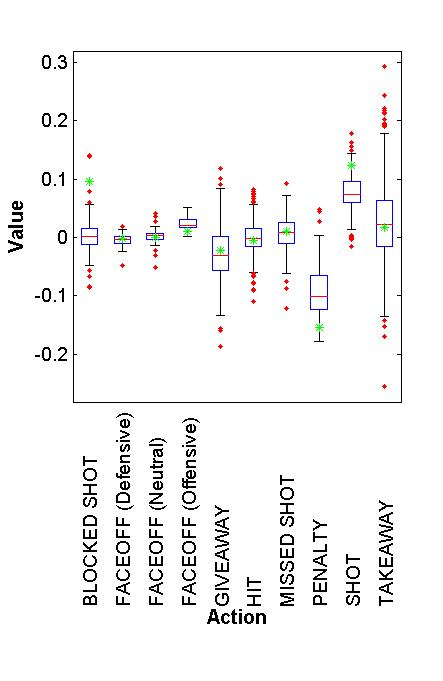
\includegraphics[width = 1.0\columnwidth]{boxplot_actionvalues3}
%\vspace{1in}
\caption{Action Value Ranges. Depending on the context, the value of an action can vary widely.}
\label{fig:boxplot-action-values}
\end{figure}

%[OS: use box plots]
%
%\begin{table}[htb]
%\caption{Lock and Schucker's Action Values (Previous Values) vs. Value Iteration Action Values}
%\label{table:action-values}
%\begin{center}
%\resizebox{1\columnwidth}{!}{
%\begin{tabular}{|c|c|c|c|c|c|}
%\hline
%\bf{Action} & \bf{Previous Value} & \multicolumn{4}{|c|}{\bf{Value Iteration}} \\ \cline{3-6}
% & & Weighted Average & Maximum & Minimum & Variance \\ \hline
%Blocked Shot & 0.0957 & 0.0004 & 0.5025 & -0.5785 & 0.0004 \\ \hline
%Faceoff (Defensive) & -0.0017 & & & & \\ \hline
%Faceoff (Neutral) & 0.0007 & & & & \\ \hline
%Faceoff (Offensive) & 0.0110 & & & & \\ \hline
%Giveaway & -0.0226 & -0.0020 & 0.5609 & -0.6065 & 0.0006 \\ \hline
%Hit & -0.0046 & -0.0001 & 0.6057 & -0.5208 & 0.0003 \\ \hline
%Missed Shot & 0.0094 & -0.0004 & 0.5890 & -0.6009 & \\ \hline
%Penalty & -0.1534 & -0.0072 & 0.1364 & -0.1920 & \\ \hline
%Shot & 0.1226 & 0.0063 & 0.5804 & -0.5008 & \\ \hline
%Takeaway & 0.0174 & 0.0018 & 0.5530 & -0.5763 & \\ \hline
%\end{tabular}
%}
%\end{center}
%\end{table}

\section{STATE STATISTICS AND VALUES: NO SEQUENCES}

general strategy: winning chance changes with goal scoring (goal diff). Goal scoring changes with penalties.  Dtree can tell you how to achieve goals or penalities locally. State backup integrates these numbers into a single one, for both goal scoring and penalty achievement. (Player ranking?)

%\begin{table*}[htb]
%\caption{Play-by-Play Sequence Contingency Table}
%\label{table:contingency-table}
%\begin{center}
%\resizebox{1\textwidth}{!}{
%\begin{tabular}{|c|c|c|c|c|c|c|c|c|}
%\hline
% \bf{Goal Differential} & \bf{Manpower Differential} & \bf{Period} & \bf{Number of Sequences} & \bf{Ends In Goal} & \bf{Ends In Penalty} & \bf{Reward = Win} & \bf{Reward = Goal} & \bf{Reward = Next Home Goal} \\ \hline
%0 & 0 & 1 & 69,358 & 4,924 & 10,014 & -0.000013206 & 0.003394622 & 0.017470455 \\ \hline
%0 & 0 & 2 & 33,976 & 2,602 & 5,233 & 0.000006222 & 0.003367201 & 0.021706954 \\ \hline
%0 & 0 & 3 & 26,741 & 1,821 & 2,787 & -0.000206337 & 0.002227779 & 0.019534592 \\ \hline
%1 & 0 & 2 & 26,482 & 2,097 & 4,221 & 0.000380054 & 0.001543053 & 0.021591389 \\ \hline
%1 & 0 & 3 & 22,826 & 1,831 & 2,666 & 0.044373381 & 0.002387631 & 0.024226838 \\ \hline
%-1 & 0 & 2 & 22,566 & 1,760 & 3,538 & -0.000382451 & 0.003115098 & 0.022845692 \\ \hline
%1 & 0 & 1 & 22,066 & 1,480 & 3,568 & 0.000000085 & 0.003423563 & 0.019661919 \\ \hline
%-1 & 0 & 3 & 19,964 & 1,565 & 2,276 & -0.046039697 & 0.001331026 & 0.021621996 \\ \hline
%-1 & 0 & 1 & 18,495 & 1,305 & 2,948 & -0.000000221 & 0.004565380 & 0.020117038 \\ \hline
%2 & 0 & 3 & 15,585 & 1,297 & 2,027 & 0.066432887 & 0.004187012 & 0.026217242 \\ \hline
%2 & 0 & 2 & 13,763 & 1,081 & 2,338 & 0.000709842 & 0.001615879 & 0.023955375 \\ \hline
%-2 & 0 & 3 & 12,314 & 962 & 1,489 & -0.071100171 & -0.001731899 & 0.023280575 \\ \hline
%-2 & 0 & 2 & 10,497 & 794 & 1,691 & -0.000812391 & 0.004713458 & 0.022603555 \\ \hline
%0 & 1 & 1 & 10,265 & 1,260 & 1,650 & -0.000000238 & 0.068621551 & 0.040057357 \\ \hline
%0 & -1 & 1 & 9,689 & 1,055 & 1,819 & -0.000000263 & -0.056201080 & 0.015560972 \\ \hline
%3 & 0 & 3 & 9,557 & 597 & 1,626 & 0.095149511 & -0.001446753 & 0.02112544 \\ \hline
%-3 & 0 & 3 & 6,715 & 410 & 1,060 & -0.100993803 & 0.003415244 & 0.021614998 \\ \hline
%0 & 0 & 4 & 6,252 & 640 & 474 & 0.000267494 & 0.005802195 & 0.034859076 \\ \hline
%0 & 1 & 2 & 6,150 & 723 & 955 & -0.000000770 & 0.058506601 & 0.043446392 \\ \hline
%3 & 0 & 2 & 5,684 & 423 & 1,051 & 0.000901368 & -0.002641091 & 0.023404221 \\ \hline
%0 & -1 & 2 & 5,679 & 672 & 970 & 0.000191954 & -0.057690825 & 0.019719806 \\ \hline
%2 & 0 & 1 & 5,347 & 345 & 931 & 0.000000315 & 0.002314936 & 0.019898360 \\ \hline
%1 & -1 & 2 & 4,836 & 606 & 753 & 0.000224084 & -0.063834184 & 0.020434313 \\ \hline
%1 & 1 & 2 & 4,682 & 579 & 805 & 0.000329883 & 0.063028993 & 0.047728124 \\ \hline
%\end{tabular}
%}
%\end{center}
%\end{table*}

%\begin{table*}[htb]
%\caption{Period Four Play-by-Play Sequence Contingency Table. Goals are more common than penalties. Penalties are more favorable for the home team.}
%\label{table:period-four-ct}
%\begin{center}
%\resizebox{1\textwidth}{!}{
%\begin{tabular}{|c|c|c|c|c|c|c|c|c|}
%\hline
% \bf{Goal Differential} & \bf{Manpower Differential} & \bf{Period} & \bf{Number of Sequences} & \bf{Ends In Goal} & \bf{Ends In Penalty} & \bf{Reward = Win} & \bf{Reward = Goal} & \bf{Reward = Next Goal} \\ \hline
% 0 & 0 & 4 & 6,252 & 640 & 474 & 0.000267494 & 0.005802195 & 0.034859076 \\ \hline
%0 & 1 & 4 & 668 & 109 & 53 & 0.004224813 & 0.131447067 & 0.097894388 \\ \hline
%0 & -1 & 4 & 564 & 87 & 54 & -0.001124987 & -0.107908279 & 0.014118699 \\ \hline
%0 & -2 & 4 & 25 & 0 & 5 & 0.000070744 & 0.001409694 & 0.014042549 \\ \hline
%0 & 2 & 4 & 23 & 2 & 1 & 0.000109450 & 0.085741439 & 0.107596947 \\ \hline
%\end{tabular}
%}
%\end{center}
%\end{table*}

%\begin{table*}[htbp]
%\caption{State Goal and Penalty Conditional Probability Table}
%\label{table:state-probabilities}
%\begin{center}
%\resizebox{1\textwidth}{!}{
%\begin{tabular}{|c|c|c|c|c|c|c|c|c|}
%\hline
% \bf{Goal Differential} & \bf{Manpower Differential} & \bf{Period} & \bf{Number of Sequences} & \bf{Probability of Home Goal} & \bf{Probability of Away Goal} & \bf{Probability of Home Penalty} & \bf{Probability of Away Penalty} \\ \hline
%0 & 0 & 1 & 69,358 & 53.43217 & 46.56783 & 49.10126 & 50.89874 \\ \hline
%0 & 0 & 2 & 33,976 & 53.99693 & 46.00307 & 48.86298 & 51.13702 \\ \hline
%0 & 0 & 3 & 26,741 & 52.60846 & 47.39154 & 48.83387 & 51.16613 \\ \hline
%1 & 0 & 2 & 26,482 & 51.40677 & 48.59323 & 51.07794 & 48.92206 \\ \hline
%1 & 0 & 3 & 22,826 & 52.70344 & 47.29656 & 51.91298 & 48.08702 \\ \hline
%-1 & 0 & 2 & 22,566 & 53.97727 & 46.02273 & 46.07123 & 53.92877 \\ \hline
%1 & 0 & 1 & 22,066 & 52.36486 & 47.63514 & 51.76570 & 48.23430 \\ \hline
%-1 & 0 & 3 & 19,964 & 50.60703 & 49.39297 & 40.64148 & 59.35852 \\ \hline
%-1 & 0 & 1 & 18,495 & 52.87356 & 47.12644 & 46.40434 & 53.59566 \\ \hline
%2 & 0 & 3 & 15,585 & 53.12259 & 46.87741 & 49.72866 & 50.27134 \\ \hline
%2 & 0 & 2 & 13,763 & 50.78631 & 49.21369 & 51.83918 & 48.16082 \\ \hline
%-2 & 0 & 3 & 12,314 & 49.58420 & 50.41580 & 43.45198 & 56.54802 \\ \hline
%-2 & 0 & 2 & 10,497 & 51.13350 & 48.86650 & 42.16440 & 57.83560 \\ \hline
%0 & 1 & 1 & 10,265 & 83.73016 & 16.26984 & 67.15152 & 32.84848 \\ \hline
%0 & -1 & 1 & 9,689 & 20.56872 & 79.43128 & 25.34360 & 74.65640 \\ \hline
%3 & 0 & 3 & 9,557 & 51.08878 & 48.91122 & 50.92251 & 49.07749 \\ \hline
%-3 & 0 & 3 & 6,715 & 53.65854 & 46.34146 & 46.69811 & 53.30189 \\ \hline
%0 & 0 & 4 & 6,252 & 52.18750 & 47.81250 & 44.72574 & 55.27426 \\ \hline
%0 & 1 & 2 & 6,150 & 79.39142 & 20.60858 & 63.66492 & 36.33508 \\ \hline
%3 & 0 & 2 & 5,684 & 50.59102 & 49.40898 & 53.47288 & 46.52712 \\ \hline
%0 & -1 & 2 & 5,679 & 22.17262 & 77.82738 & 30.82474 & 69.17526 \\ \hline
%2 & 0 & 1 & 5,347 & 52.46377 & 47.53623 & 54.45757 & 45.54243 \\ \hline
%1 & -1 & 2 & 4,836 & 21.12211 & 78.87789 & 35.72377 & 64.27623 \\ \hline
%1 & 1 & 2 & 4,682 & 81.17444 & 18.82556 & 65.21739 & 34.78261 \\ \hline
%\end{tabular}
%}
%\end{center}
%\end{table*}

%\begin{table*}[htb]
%\caption{Even-Strength State Conditional Probability Table. The away team is more likely to receive a penalty when the away team is leading or the goals are even. The leveling bias is stronger against the away team. There appears to be a relationship between home team bias and the period.}
%\label{table:even-strength-state-probabilities}
%\begin{center}
%\resizebox{1\textwidth}{!}{
%\begin{tabular}{|c|c|c|c|c|c|c|c|c|}
%\hline
% \bf{Goal Differential} & \bf{Period} & \bf{Number of Sequences} & \bf{Difference in Conditional Probability of Goal} & \bf{Difference in Conditional Probability of Penalty} \\ \hline
%-3 & 3 & 6,715 & 7.31708 & -6.60378 \\ \hline
%-2 & 3 & 12,314 & -0.83160 & -13.09604 \\ \hline
%-2 & 2 & 10,497 & 2.26700 & -15.67120 \\ \hline
%-1 & 3 & 19,964 & 1.21406 & -18.71704 \\ \hline
%-1 & 2 & 22,566 & 7.95454 & -7.85754 \\ \hline
%-1 & 1 & 18,495 & 5.74712 & -7.19132 \\ \hline
%0 & 4 & 6,252 & 4.37500 & -10.54852 \\ \hline
%0 & 3 & 26,741 & 5.21692 & -2.33226 \\ \hline
%0 & 2 & 33,976 & 7.99386 & -2.27404 \\ \hline
%0 & 1 & 69,358 & 6.86434 & -1.79748 \\ \hline
%1 & 3 & 22,826 & 5.40688 & 3.82596 \\ \hline
%1 & 2 & 26,482 & 2.81354 & 2.15588 \\ \hline
%1 & 1 & 22,066 & 4.72972 & 3.53140 \\ \hline
%2 & 3 & 15,585 & 6.24518 & -0.54268 \\ \hline
%2 & 2 & 13,763 & 1.57262 & 3.67836 \\ \hline
%2 & 1 & 5,347 & 4.92754 & 8.91514 \\ \hline
%3 & 3 & 9,557 & 2.17756 & 1.84502 \\ \hline
%3 & 2 & 5,684 & 1.18204 & 6.94576 \\ \hline
%\end{tabular}
%}
%\end{center}
%\end{table*}

%\begin{table*}[htb]
%\caption{Penalty State Conditional Probability Table. Bias to call a penalty against the team on the power play decreases as the period number increases. There is an obvious benefit to being on the powerplay as observed by the conditional probability of scoring.}
%\label{table:penalty-state-probabilities}
%\begin{center}
%\resizebox{1\textwidth}{!}{
%\begin{tabular}{|c|c|c|c|c|c|c|c|c|}
%\hline
% \bf{Goal Differential} & \bf{Manpower Differential} & \bf{Period} & \bf{Number of Sequences} & \bf{Difference in Conditional Probability of Goal} & \bf{Difference in Conditional Probability of Penalty} \\ \hline
%0 & -1 & 1 & 9,689 & -58.86256 & -49.31280 \\ \hline
%1 & -1 & 1 & 3,741 & -58.20106 & -45.84528 \\ \hline
%-1 & -1 & 2 & 3,649 & -56.06408 & -40.75286 \\ \hline
%0 & -1 & 2 & 5,679 & -55.65476 & -38.35052 \\ \hline
%1 & -1 & 2 & 4,836 & -57.75578 & -28.55246 \\ \hline
%0 & -1 & 3 & 3,197 & -62.13334 & -37.40832 \\ \hline
%2 & -1 & 3 & 3,342 & -9.91380 & -18.56288 \\ \hline
%1 & -1 & 3 & 4,427 & -18.84550 & -22.01492 \\ \hline
%0 & 1 & 1 & 10,265 & 67.46032 & 34.30304 \\ \hline
%1 & 1 & 1 & 3,611 & 72.06982 & 36.34946 \\ \hline
%-1 & 1 & 1 & 3,301 & 66.31016 & 23.82812 \\ \hline
%1 & 1 & 2 & 4,682 & 62.34888 & 30.43478 \\ \hline
%-1 & 1 & 2 & 4,296 & 60.00000 & 23.74100 \\ \hline
%0 & 1 & 2 & 6,150 & 58.78284 & 27.32984 \\ \hline
%-1 & 1 & 3 & 4,320 & 29.35484 & 16.98842 \\ \hline
%0 & 1 & 3 & 3,501 & 66.66666 & 27.92362 \\ \hline
%\end{tabular}
%}
%\end{center}
%\end{table*}

insert contingency table of sequences based on
(goal differential, manpower differential, period). with the following fields:

sequence count.
ends-in-goal-count. Home/Away.
ends-in-penalty-count. Home/Away.
Value for different reward functions. Computed with sequences in states.
1) Reward = win. 2) reward = goal. 3) reward = next goal.


\subsection{SEQUENCES}


\subsection{VALUE ITERATION}

\subsection{REWARD FUNCTION = WIN}

Back up wins. Show that after conditioning, agrees with observed frequency. [maybe other interesting states as well.]

\subsection{REWARD FUNCTION = GOAL}

Back up computes expected goals. How to evaluate?

\subsection{REWARD FUNCTION = NEXT GOAL}

When a goal is scored, finish process. Interpretation: probability that next goal is scored by team. Evaluate using a separate tree for data counts.

\section{APPLICATIONS}



%\subsection{HYPOTHESES}

%A nice way to structure this section and to engage the referees is to give a list of what you want to establish through your experiments, before you give the details of your experiments. This usually also clarifies things for yourself. Hopefully you have more interesting hypotheses to test than ``I can find some datasets on which the predictive accuracy of my system is higher than that of some previous methods.''

\subsection{HARDWARE}

Data was obtained from \url{http://www.nhl.com} using the Selenium WebDriver with Python 2.7.6 \citep{Salunke2014} on a 64-bit Ubuntu 14.0.4 LTS Virtual Machine with 4.8GB RAM and a Intel Core i7-2670QM CPU @ 2.20GHz $\times$ 8. Data table construction and value iteration was performed using Java Version 8 Update 25 on 64-bit Windows 7 Home Premium with 12GB RAM and a Intel Core i7-2670QM CPU @ 2.20GHz $\times$ 8.

%Describe briefly your set-up, e.g. RAM, Processor, programming language.

\subsection{DATASETS}



%Outline the datasets that you are using. Highlight interesting aspects. Give summary statistics (e.g., data set sizes). Are they real-world or synthetic?

%It can be a good idea to present your data in terms of sample training and test sets.

\subsection{METHODS COMPARED}

%List all of the methods. Make sure you explain which methods are yours and which were proposed by other researchers. Explain settings of methods, and why you chose them.

\subsection{PERFORMANCE MEASURES}

%Explain what you are measuring (e.g., runtime, accuracy) etc. More is better. How are you computing the numbers? E.g., with cross-validation, taking averages? Usually referees like you to add error bars or standard deviations.

\subsection{RESULTS}

%You need to report results for triples of (method, datasets, metric). This kind of three-dimensional setting is not easy to translate into graphs but you should try. It's best to try and find graphs that support your points; refer back to the hypotheses listed above. I suggest importing  your data into a spreadsheet program, which allows you to produce many charts. Also, there are macros that convert Excel tables into latex tables. This saves you a lot of the pain of producing Latex tables. Avoid color graphs because referees may be printing on black and white, and in any case the conference proceedings won't be in color.

\section{CONCLUSION}

It would be interesting to see the effect of shift changes, that is, when a player enters or leaves the ice, within action event sequences. As such, finding an efficient way to make use the available temporal data alongside the Markov Decision Process would be an interesting study. Goalies do not participate in many recorded events, it is difficult to evaluate goalies with this model, and extension methods for evaluating goaltenders are left as future work. Learning what context features perform better than others could also be an interesting study. For example, is using shots without any descriptors enough, or should shots be augmented with the shot location and shot type as in \citep{Krzywicki2005}?

%This should be a summary of the main points and what your findings were. Repeat why these results are significant. Often it's a good idea to add some avenues for future work. Often reviewers think ``yes, but you should also have done xyz''. If you can guess what xyz is, you can mention it as an avenue for future work, and then you have shown that you did think of xyz and you acknowledge its importance.

%\section{REFERENCES} Students don't pay nearly enough attention to references. Referees get turned off if the references are incomplete, hard to read, etc., especially if this is is the case for citations to their own work.

%\section{FIRST LEVEL HEADINGS}
%
%First level headings are all caps, flush left, bold and in point size
%12. One line space before the first level heading and 1/2~line space
%after the first level heading.
%
%\subsection{SECOND LEVEL HEADING}
%
%Second level headings must be flush left, all caps, bold and in point
%size 10. One line space before the second level heading and 1/2~line
%space after the second level heading.
%
%\subsubsection{Third Level Heading}
%
%Third level headings must be flush left, initial caps, bold, and in
%point size 10.  One line space before the third level heading and
%1/2~line space after the third level heading.
%
%\vskip .5pc
%Fourth Level Heading
%
%Fourth level headings must be flush left and initial caps.
%One line space before the fourth level heading and 1/2~line space
%after the fourth level heading.

%\subsection{CITATIONS, FIGURES, REFERENCES}


%\subsubsection{Citations in Text}
%
%Citations within the text should include the author's last name and
%year, e.g., (Cheesman, 1985). Reference style should follow the style
%that you are used to using, as long as the citation style is
%consistent.
%
%For the original submission, take care not to reveal the authors' identity through
%the manner in which one's own previous work is cited.  For example, writing
%``In (Bovik, 1970), we studied the problem of AI'' would be inappropriate, as
%it reveals the author's identity.  Instead, write ``(Bovik, 1970) studied the
%problem of AI.''

%\subsubsection{Footnotes}
%
%Indicate footnotes with a number\footnote{Sample of the first
%footnote} in the text. Use 8 point type for footnotes.  Place the
%footnotes at the bottom of the page on which they appear.  Precede the
%footnote with a 0.5 point horizontal rule 1~inch (6~picas)
%long.\footnote{Sample of the second footnote}

%\subsubsection{Figures}
%
%All artwork must be centered, neat, clean, and legible. Figure number
%and caption always appear below the figure.  Leave 2 line spaces
%between the figure and the caption. The figure caption is initial caps
%and each figure numbered consecutively.
%
%Make sure that the figure caption does not get separated from the
%figure. Leave extra white space at the bottom of the page rather than
%splitting the figure and figure caption.
%\begin{figure}[ht]
%\vspace{1in}
%\caption{Sample Figure Caption}
%\end{figure}

%\subsubsection{Tables}
%
%All tables must be centered, neat, clean, and legible. Table number
%and title always appear above the table.  %See
%Table~\ref{sample-table}.
%
%One line space before the table title, one line space after the table
%title, and one line space after the table. The table title must be
%initial caps and each table numbered consecutively.
%
%\begin{table}[h]
%\caption{Sample Table Title}
%\label{sample-table}
%\begin{center}
%\begin{tabular}{ll}
%\multicolumn{1}{c}{\bf PART}  &\multicolumn{1}{c}{\bf DESCRIPTION} \\
%\hline \\
%Dendrite         &Input terminal \\
%Axon             &Output terminal \\
%Soma             &Cell body (contains cell nucleus) \\
%\end{tabular}
%\end{center}
%\end{table}

\newpage

%\subsubsection*{Acknowledgements}

%Use unnumbered third level headings for the acknowledgements title.
%All acknowledgements go at the end of the paper.


%\subsubsection*{References}

%References follow the acknowledgements.  Use unnumbered third level
%heading for the references title.  Any choice of citation style is
%acceptable as long as you are consistent.

%NOTE: NEED TO USE CORRECT REFERENCES HEADER
\bibliographystyle{apalike}
\renewcommand\bibsection{\subsubsection*{\refname}}
\bibliography{master}


%J.~Alspector, B.~Gupta, and R.~B.~Allen  (1989). Performance of a
%stochastic learning microchip.  In D. S. Touretzky (ed.), {\it Advances
%in Neural Information Processing Systems 1}, 748-760.  San Mateo, Calif.:
%Morgan Kaufmann.

%F.~Rosenblatt (1962). {\it Principles of Neurodynamics.} Washington,
%D.C.: Spartan Books.

%G.~Tesauro (1989). Neurogammon wins computer Olympiad.  {\it Neural
%Computation} {\bf 1}(3):321-323.

\end{document}
